\documentclass[titlepage]{article}
\usepackage{babel}
\usepackage{amsmath}
\usepackage{amssymb}
\usepackage{amsthm}
\usepackage{multicol} %spalten in seite
\usepackage{graphicx} %bilder einfügen
\usepackage[normalem]{ulem} %durchstreichen
\usepackage{tabto} %tabulator mit \tab
\usepackage{hyperref}
\usepackage{tikz}
\usetikzlibrary{shapes.geometric}
\usepackage{wasysym}
\usepackage{bbm}
\usepackage{bbold}
\usepackage{xcolor}
\usepackage[T1]{fontenc}
\usepackage{mathrsfs}  
\usepackage[utf8]{inputenc}
\usepackage{listings} %quellcode
\pagestyle{plain}
\pagenumbering{arabic}
\renewcommand{\arraystretch}{1.3} %vertikaler abstand von tabellen
\newcommand{\n}{\newline}
\usepackage[left=20mm, right=15mm, top=25mm, bottom=7mm, paper=a4paper]{geometry}
\renewcommand{\contentsname}{Inhaltsverzeichnis}

\newcommand{\K}{\mathbb{K}}
\newcommand{\C}{\mathbb{C}}
\newcommand{\N}{\mathbb{N}}
\newcommand{\Q}{\mathbb{Q}}
\newcommand{\R}{\mathbb{R}}
\newcommand{\1}{\mathbb{1}}
\newcommand{\0}{\mathbb{0}}
\newcommand{\Z}{\mathbb{Z}}

\begin{document}
	
	\begin{center}
		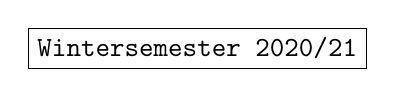
\begin{tikzpicture}
			\draw (0,0) node[draw, rectangle]{\texttt{Wintersemester 2020/21}};
		\end{tikzpicture}
		\hrulefill\\
		\begin{center}
			\LARGE Diskrete Strukturen - Übung 08 \normalsize\\
		\end{center}
		\hrulefill
		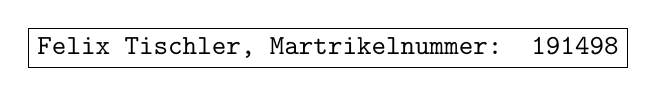
\begin{tikzpicture}
			\draw (0,0) node[draw, rectangle]{\texttt{Felix Tischler, Martrikelnummer: 191498}};
		\end{tikzpicture}
		\date{\today}
	\end{center}
	
	\part*{Aussagen und Formeln}
	\section*{1.) \textit{$Sind$ $die$ $folgenden$ $Schlussfolgerungen$ $richtig$ $oder$ $falsch?$ $Formalisieren$ $Sie$ $und$ $\ddot uberpr\ddot ufen$ $Sie,$ $ob$ $die$ $Gesamtheit$ $der$ $jeweiligen$ $Annahmen$ $die$ $angegebene$ $Konsequenz$ $zur$ $Folge$ $hat.$}}
		\subsection*{a) \textit{$Anton$ $ist$ $ein$ $L\ddot ugner$ $oder$ $Bertram$ $war$ $in$ $Berlin$ $oder$ $Claudius$ $ist$ $kein$ $Erpresser.$ $Wenn$ $Bertram$ $nicht$ $in$ $Berlin$ $war,$ $dann$ $ist$ $Anton$ $kein$ $L\ddot ugner$ $oder$ $Claudius$ $ist$ $ein$ $Erpresser.$ $Folglich$ $muss$ $Bertram$ $in$ $Berlin$ $gewesen$ $sein.$}}
			\begin{enumerate}
				\item Anton ist Lügner $\vee$ Betram war in Berlin $\vee$ Claudius ist $\neg$Erpresser
				\item Betram war $\neg$in Berlin $\Rightarrow$(Anton ist $\neg$Lügner $\vee$ Claudius ist kein Erpresser)
				\item $\Longrightarrow$ Betram war in Berlin
			\end{enumerate}
		Sei \textit{A:= Anton ist ein Lügner}, \textit{B:= Betram war in Berlin} und \textit{C:= Claudius ist ein Erpresser}.
			\begin{align*}
				\underbrace{(A\vee B\vee C)}_{x1}\wedge\underbrace{(\neg B\Rightarrow(\neg A\vee\neg C))}_{x2}\Rightarrow B
			\end{align*}
		Angenommen es sei $\neg B$. x1 und x2 wären weiterhin erfüllt und aus ihnen würde $B$ folgen. Also führt die Annahme $\neg B$ zu $B$ und dies ist ein Widerspruch. \textcolor{red}{\lightning}
		\subsection*{b) \textit{$Wenn$ $der$ $Staatshaushalt$ $nicht$ $gek\ddot urzt$ $wird,$ $dann$ $bleiben$ $die$ $Preise$ $stabil$ $dann$ $und$ $nur$ $dann,$ $wenn$ $die$ $Steuern$ $erh\ddot oht$ $werden.$ $Der$ $Staatshaushalt$ $wird$ $nicht$ $gek\ddot urzt,$ $wenn$ $die$ $Steuern$ $erh\ddot oht$ $werden.$ $Wenn$ $die$ $Preise$ $stabil$ $bleiben,$ $werden$ $die$ $Steuern$ $nicht$ $erh\ddot oht.$ $Folglich$ $werden$ $die$ $Steuern$ $nicht$ $erh\ddot oht.$}}
			\begin{enumerate}
				\item Staatshaushalt wird $\neg$gekürzt $\Rightarrow$ Preise bleiben stabil $\Leftrightarrow$ Steuern werden erhöht
				\item Staatshaushalt wird $\neg$gekürzt $\Leftarrow$ Steuern werden erhöht
				\item Preise bleiben stabil $\Rightarrow$ Steuern werden $\neg$erhöht
				\item $\Longrightarrow$ Steuern werden $\neg$erhöht
			\end{enumerate}
		Sei \textit{A:= Staatshaushalt wird nicht gekürzt}, \textit{B:= Preise bleiben stabil} und \textit{C:= Steuern werden erhöht}.
		\begin{align*}
			\underbrace{((A\Rightarrow B)\Leftrightarrow C)}_{x1}\wedge\underbrace{( C\Rightarrow A)}_{x2}\wedge\underbrace{(B\Rightarrow\neg C)}_{x3}\Rightarrow\neg C
		\end{align*}
		
		
			\begin{table}[h]
				\scalebox{1}{
				\begin{tabular}{ccc|cccccc}
					A&B&C&$A\Rightarrow B$&$\neg C$&x1&x2&x3&(x1 $\land$ x2 $\land$ x3) $\Rightarrow\neg C$\\\hline
					0&0&0&1&1&0&1&1&1\\
					0&0&1&1&0&1&0&1&1\\
					0&1&0&1&1&0&1&1&1\\
					0&1&1&1&0&1&0&0&1\\
					1&0&0&0&1&1&1&1&1\\
					1&0&1&0&0&0&1&1&1\\
					1&1&0&1&1&1&1&1&1\\
					1&1&1&1&0&1&1&0&1
				\end{tabular}
				}
			\end{table}
		D.h. unabhängig von A,B oder C ist die Aussage $(x1\land x2\land x3)\Rightarrow\neg C$ immer wahr.\qed
	
	\newpage
	\section*{2.)}
		\subsection*{a) \textit{$Bestimmen$ $Sie$ $die$ $zugeh\ddot orige$ $Boolesche$ $Funktion$ $f_F$ $f\ddot ur$ $folgende$ $aussagenlogischen$ $Formel:$}}
		\begin{align*}
			F=\underbrace{((C\rightarrow\neg A)\wedge(\underbrace{(A\wedge\neg B)\rightarrow(B\vee\neg C)}_*))}_{**}\leftrightarrow\lnot(A\wedge B)
		\end{align*}
			\begin{table}[h]
				\begin{tabular}{ccc||cccccccc}
					A&B&C&$A\wedge B$&$\neg A$&$C\rightarrow\neg A$&$A\wedge\neg B$&$B\vee\neg C$&*&**&$((C\rightarrow\neg A)\wedge((A\wedge\neg B)\rightarrow(B\vee\neg C)))\leftrightarrow\lnot(A\wedge B)$\\\hline
					0&0&0&0&1&1&0&1&1&1&1\\
					0&0&1&0&1&1&0&0&1&1&1\\
					0&1&0&0&1&1&0&1&1&1&1\\
					0&1&1&0&1&1&0&1&1&1&1\\
					1&0&0&0&0&1&1&1&1&1&1\\
					1&0&1&0&0&0&1&0&0&0&0\\
					1&1&0&1&0&1&0&1&1&1&0\\
					1&1&1&1&0&0&0&1&1&0&1
				\end{tabular}
			\end{table}
		
		\subsection*{b) \textit{$Bestimmen$ $Sie$ $eine$ $aussagenlogische$ $Formel$ $G,$ $in$ $der$ $die$ $Atome$ $A,$ $B$ $und$ $C$ $vorkommen$ $(und$ $keine$ $weiteren),$ $so$ $dass$ $die$ $zugeh\ddot orige$ $Wahrheitswerttabelle$ $bei$ $der$ $von$ $uns$ $verwendeten$ $Standardanordnung$ $als$ $Ergebniseintrag$ $von$ $oben$ $nach$ $unten$ $das$ $Tupel$ $(1,1,1,0,0,1,1,1)$ $enthält.$}}
			\begin{table}[h]
				\begin{tabular}{ccc|c}
					A&B&C&$(\overline{A}\land\overline{B}\land\overline{C})\lor(\overline{A}\land\overline{B}\land C)\lor(\overline{A}\land B\land\overline{C})\lor(A\land\overline{B}\land C)\lor(A\land B\land\overline{C})\lor(A\land B\land C)$\\\hline
					0&0&0&1\\
					0&0&1&1\\
					0&1&0&1\\
					0&1&1&0\\
					1&0&0&0\\
					1&0&1&1\\
					1&1&0&1\\
					1&1&1&1
				\end{tabular}
			\end{table}
		D.h. z.B. $F:=(\overline{A}\land\overline{B}\land\overline{C})\lor(\overline{A}\land\overline{B}\land C)\lor(\overline{A}\land B\land\overline{C})\lor(A\land\overline{B}\land C)\lor(A\land B\land\overline{C})\lor(A\land B\land C)$
		
	\section*{3.) \textit{$Geben$ $Sie$ $eine$ $aussagenlogische$ $Formel$ $H$ $mit$ $den$ $Atomen$ $A,$ $B$ $und$ $C$ $an,$ $die$ $die$ $folgende$ $Eigenschaft$ $f\ddot ur$ $alle$ $Belegungen$ $\beta$ $erf\ddot ullt:$ $\ddot Andert$ $man$ $genau$ $einen$ $der$ $Werte$ $\beta(A)$ $bzw.$ $\beta(B)$ $bzw.$ $\beta(C),$ $dann$ $\ddot andert$ $sich$ $auch$ $der$ $Wert$ $I_{\beta}(H).$}}
	.
		\begin{table}[h]
			\begin{tabular}{ccc|c}
				A&B&C&$I_{\beta}(H)$\\\hline
				0&0&0&0\\
				0&0&1&1\\
				0&1&0&1\\
				0&1&1&0\\
				1&0&0&1\\
				1&0&1&0\\
				1&1&0&0\\
				1&1&1&1
			\end{tabular}\quad\quad\quad\quad
			$H:=(\overline{A}\land\overline{B}\land C)\lor(\overline{A}\land B\land\overline{C})\lor(A\land\overline{B}\land\overline{C})\lor(A\land B\land C)$
		\end{table}
	
	\section*{4.) \textit{$Beweisen$ $Sie,$ $dass$ $die$ $folgenden$ $vier$ $Aussagen$ $äquivalent$ $sind:$}}
		\subsection*{a) \textit{$Es$ $gibt$ $eine$ $Formel$ $G,$ $so$ $das$ $gilt:$ $G$ $ist$ $Folgerung$ $aus$ $F$ $und$ $\neg G$ $ist$ $Folgerung$ $aus$ $F.$ $(Dies$ $ist$ $die$ $Definition$ $f \ddot ur:$ $F$ $ist$ $kontradiktorisch.)$}}
		\subsection*{b) \textit{$(A\wedge\neg A)$ $ist$ $Folgerung$ $aus$ $F.$}}
		\subsection*{c) \textit{$Jede$ $beliebige$ $Formel$ $H$ $ist$ $Folgerung$ $aus$ $F.$}}
		\subsection*{d) \textit{$F$ $ist$ $nicht$ $erf\ddot ullbar.$ $(Dies$ $ist$ $die$ $Definition$ $f \ddot ur:$ $F$ $ist$ $unerf\ddot ullbar.)$}}
		
		Die vier Aussagen wurden zunächst umgeschrieben:
		\begin{enumerate}
			\item []
			\begin{enumerate}
				\item $I_{\beta}(F)\le I_{\beta}(G)\land I_{\beta}(F)\le I_{\beta}(\neg G)$
				\item $I_{\beta}(F)\le I_{\beta}(A\land\neg A)$
				\item $I_{\beta}(F)\le I_{\beta}(H)$
				\item $I_{\beta}(F)=0$
			\end{enumerate}
			\begin{align*}
				(a)&\leftrightarrow (F\rightarrow G)\text{ Tautologie }\land(\lnot F\rightarrow G)\text{ Tautologie }\\
				&\leftrightarrow[(F\rightarrow G)\land(\lnot F\rightarrow G)]\text{ Tautologie}\\
				&\leftrightarrow[(\lnot F\lor G)\land(\lnot F\lor\lnot G)]\text{ Tautologie}\\
				&\leftrightarrow\lnot F\lor(G\land\lnot G)\text{ Tautologie}\\
				&\leftrightarrow\underbrace{\lnot F\text{ Tautologie}}_*\\\\
				(b)&\leftrightarrow F\rightarrow(A\land\lnot A)\text{ Tautologie}\\
				&\leftrightarrow\lnot F\lor(A\land\lnot A)\text{ Tautologie}\\
				&\leftrightarrow{*}\\\\
				(c)&\leftrightarrow F\rightarrow H\text{ Tautologie}\\
				&\leftrightarrow\lnot F\lor H\text{ Tautologie}\\
				&\leftrightarrow{*}\\\\
				(d)&\leftrightarrow I_{\beta}(F)=0\\
				&\leftrightarrow I_{\beta}(\lnot F)=1\\
				&\leftrightarrow{*}
			\end{align*}\qed
		\end{enumerate}

\end{document}
